%\subsection{Simulation framework}

The simulation program of ATLAS experiment is integrated into the ATLAS software framework called \textit{Athena}~\cite{atlas:athena},
which uses Python as an interpreter language and object-oriented script to load C++ objects and algorithms.
The ATLAS simulation data flow is shown in figure~\ref{fig:frame_overview},
where the square-cornered boxes represents algorithms and applications to be run and round-cornered boxes denote data objects.
\begin{figure}[!htb]
  \centering
  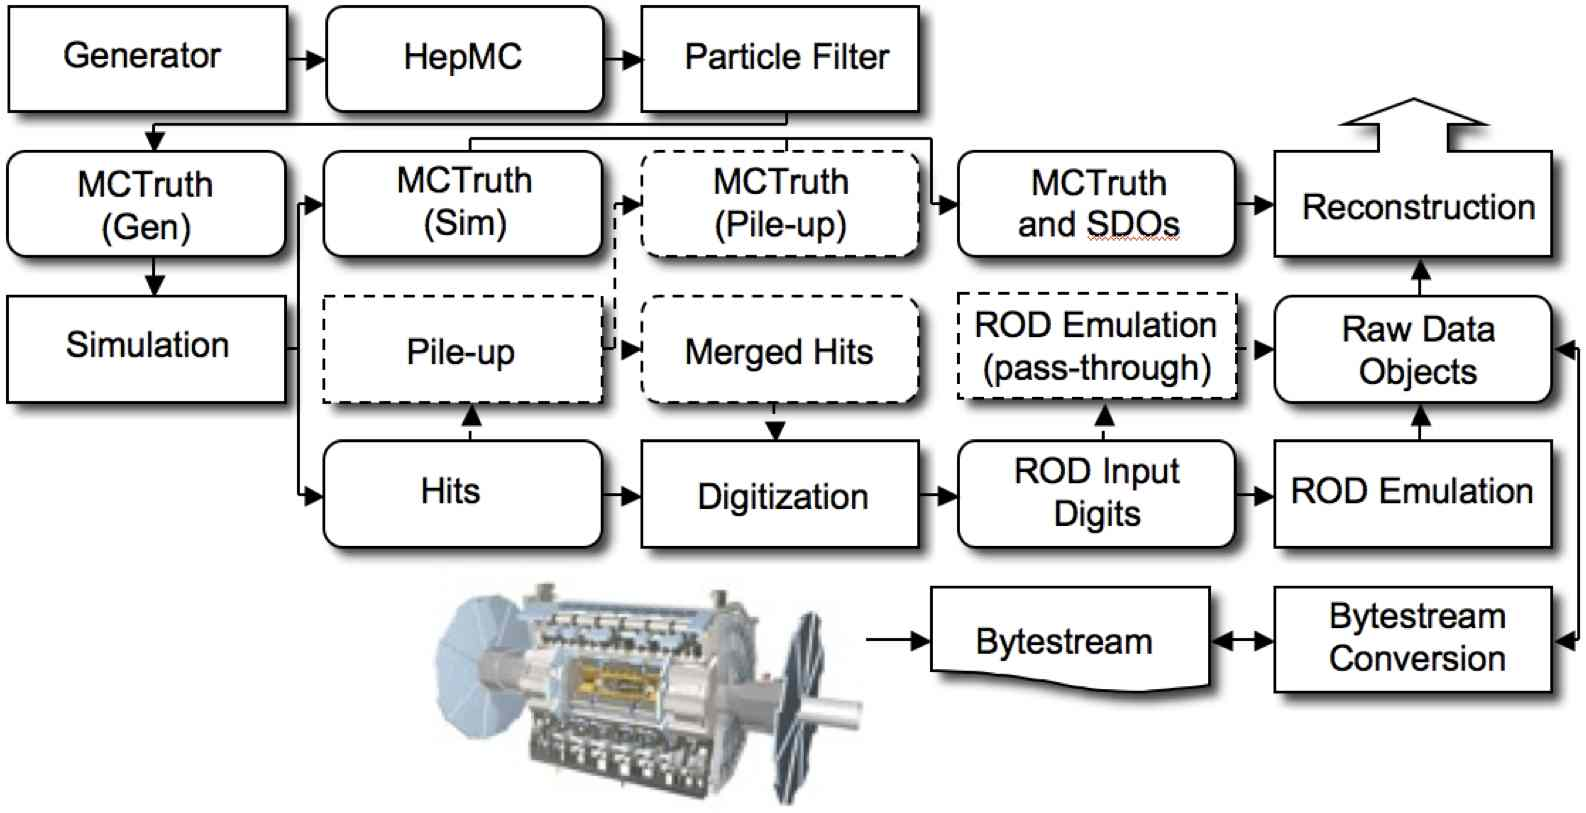
\includegraphics[width=1.0\textwidth]{figures/Simulation/outline_atalsSimulation_v2.png}
  \caption{Schematic diagram of the ATLAS simulation software~\cite{Aad:2010ah}.}
  \label{fig:frame_overview}
\end{figure}

First of all, events are produced by MC generators in standard HepMC format and then read into the detector simulation.
During the simulation, particles are propagated through the full ATLAS detector whose configurations can be set by users via GEANT4 toolkit.
%The energies deposited in the sensitive regions of the detector are recorded as \textit{hits} that contains the total energy deposition, position and time, and are written to a simulation hit file.
The \textit{hits} informations, obtained from the energies deposited in the sensitive regions of the detector, containing the total value of energy deposition, time and position, are written into hit files.
In the meatime, the events in ``truth" format are also recorded to contain the history of the interactions from the generator, including incoming and outgoing particles.
Simulated Data Objects (SDOs) are created from truth, which are maps between hits in sensitive portions of the detector and truth information of particles in simulation.
The hit files are then sent to digitization, which constructs ``digits" written into Raw Data Object (RDO) file used for reconstruction.

In conclusion, there are three main parts of framework: \textit{Generation}, \textit{Simulation} and \textit{Digitization}.
More details are given as below:

\textbf{Event generation}

As shown in figure~\ref{fig:mc_event_structure}~\cite{Hoche:2014rga}, at hadron colliders, multiple scattering and rescattering effects arise, which needs to be simulated by Monte Carlo (MC) event generators to reflect the full complexity of those event structures.
Several MC event generators can be used to generate events in HepMC format.
The events can be filtered at generation time with some certain requirements (eg. decay channel or missing energy above a certain threshold).
The generator is in charge of any prompt decays, like W and Z bosons decays, and all ``stable" particles expected to propagate through the detector are stored. 
During the generation steps, the detector effects are ignored and only immediate decays are considered.

There are several MC generators that have been widely used with general purpose, including \textsc{Sherpa}~\cite{Gleisberg_2009}, \textsc{Herwig++}~\cite{Bahr2008}, \textsc{PowhegBox}~\cite{Nason:2004rx}, \textsc{MC@NLO}~\cite{Frixione_2002} and \textsc{Pythia8}~\cite{Sjostrand:2007gs}.

\begin{figure}[!htb]
  \centering
  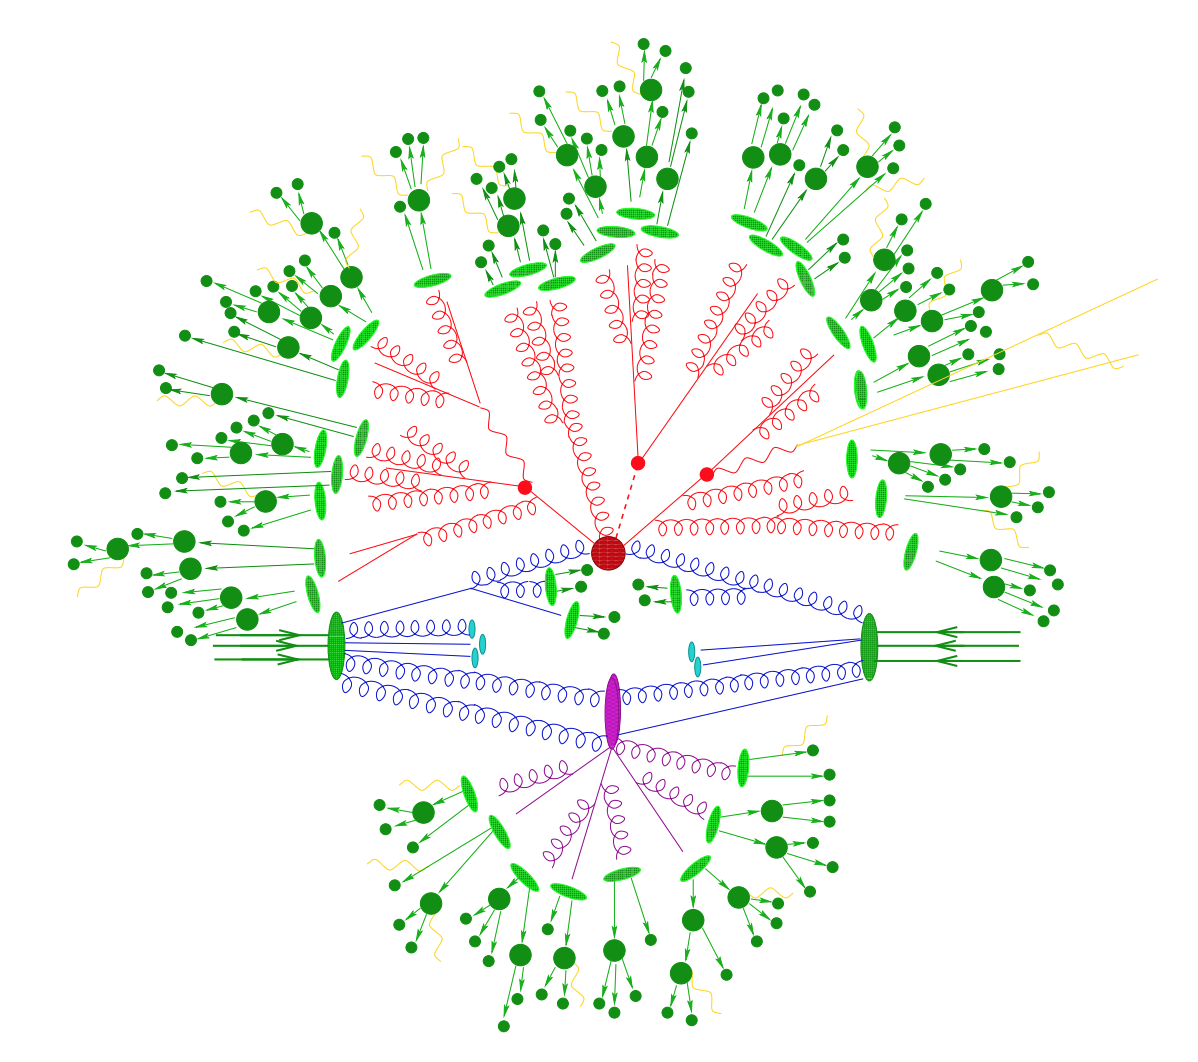
\includegraphics[width=0.7\textwidth]{figures/Simulation/mc_event_structure.png}
  \caption{Schematic of a hadron-hadron collision event simulated by MC generator. The red blob in center denotes the hard collision, surrounded by tree-like structures denoting Bremsstrahlung from Parton Showers. The purple blob is a secondary hard scattering event. The light green blobs represent the parton-to-hadron transitions while the dark green blobs stand for hadron decays. The yellow lines indicate soft photon radiations.}
  \label{fig:mc_event_structure}
\end{figure}

\textbf{Simulation}

GEANT4 is used as standard simulation toolkit for the ATLAS experiment, which transports physics particles through the detector's geometry.
During the generation level, the entire connected chain of the HepMC event is stored as the Monte Carlo truth. 
Only the stable particles are read into GEANT4 for further simulation and selection, and transformations can be applied to these events to select certain processes.
During the simulation, many secondary tracks can be produced, therefore only information from the interactions of interest are stored, including the incoming particles, step sequence, vertex as well as outgoing particles.
The output of GEANT4 is called \textit{hit file}, containing metadata including the simulation configuration, all requested truth information and the hit informations of each subdetector.

Since the standard ATLAS detector simulation cost very large computing resources to accurately model the complex detector geometry and physics descriptions, some fast simulation programss are developed according to different user purpose.
Some popular fast-sim toolkits include \textit{Fast G4 Simulation}~\cite{Barberio:2007gba}, \textit{ATLFAST-I}~\cite{Richter-Was:683751} and \textit{ATLFAST-II}~\cite{Edmonds:1091969}.

\textbf{Digitization}

The hit informations from detector simulation by GEANT4 
%including hard scattering signal, minimum bias, beam halo, beam gas and cavern background events, 
are then sent into the digitization procedure to be converted into detector response called ``digits".
Before producing the detector signal formart, events can be overlaid at a user-specified rate, called ``pile-up".
The simulation of pile-up can be done during digitization to save the CPU time.
At this stage, the detector noise and the first level trigger that implemented with hardware on the real detector are added into events.
Firstly, the ``digits" inputs are constructed and passed to the simulated readout drivers (RODs) as in the detector electronics.
The output of this step are written out as Raw Data Object (RDO) file.
In addition, the digitization algorithms can also produce Simulated Data Objects (SDOs), which contain information about all the particles, noise and the amount of energy that contributed to the signal. 
Then all information are sent into reconstruction level described in next subsection.
